\documentclass[a4paper]{article}
\usepackage[T1]{fontenc}			% \chapter package
\usepackage[english]{babel}
\usepackage[english]{isodate}  		% date format
\usepackage{graphicx}				% manage images
\usepackage{amsfonts}
\usepackage{booktabs}				% high quality tables
\usepackage{amsmath}				% math package
\usepackage{amssymb}				% another math package (e.g. \nexists)
\usepackage{bm}                     % bold math symbols
\usepackage{mathtools}				% emphasize equations
\usepackage{stmaryrd} 				% '\llbracket' and '\rrbracket'
\usepackage{amsthm}					% better theorems
\usepackage{enumitem}				% manage list
\usepackage{pifont}					% nice itemize
\usepackage{cancel}					% cancel math equations
\usepackage{caption}				% custom caption
\usepackage[]{mdframed}				% box text
\usepackage{multirow}				% more lines in a table
\usepackage{textcomp, gensymb}		% degree symbol
\usepackage[x11names]{xcolor}		% RGB color
\usepackage[many]{tcolorbox}		% colorful box
\usepackage{multicol}				% more rows in a table (used for the lists)
\usepackage{listings}
\usepackage{url}
\usepackage{qrcode}
\usepackage{fontawesome5}
\usepackage{ragged2e}
\usepackage{cite}                   % references
\usepackage{imakeidx}               % index
\makeindex[program=makeindex, columns=1,
           title=Index, 
           intoc,
           options={-s index-style.ist}]
\usepackage{fancyhdr}

%\pdfcompresslevel=0
%\pdfobjcompresslevel=0

\definecolor{codegreen}{rgb}{0,0.6,0}
\definecolor{codegray}{rgb}{0.5,0.5,0.5}
\definecolor{codepurple}{rgb}{0.58,0,0.82}
\definecolor{backcolour}{rgb}{0.95,0.95,0.92}
\lstdefinestyle{mystyle}{
    backgroundcolor=\color{backcolour},
    commentstyle=\color{codegreen},
    keywordstyle=\color{magenta},
    numberstyle=\tiny\color{codegray},
    stringstyle=\color{codepurple},
    basicstyle=\ttfamily\footnotesize,
    breakatwhitespace=false,
    breaklines=true,
    captionpos=b,
    keepspaces=true,
    numbers=left,
    numbersep=5pt,
    showspaces=false,
    showstringspaces=false,
    showtabs=false,
    tabsize=2
}
\lstset{style=mystyle}


% thanks Mico: https://tex.stackexchange.com/a/60218/312896
\makeatletter
\renewcommand\paragraph{\@startsection{paragraph}{4}{\z@}%
            {-2.5ex\@plus -1ex \@minus -.25ex}%
            {1.25ex \@plus .25ex}%
            {\normalfont\normalsize\bfseries}}
\makeatother
\setcounter{secnumdepth}{4} % how many sectioning levels to assign numbers to
\setcounter{tocdepth}{4}    % how many sectioning levels to show in ToC


% draw a frame around given text
\newcommand{\framedtext}[1]{%
	\par%
	\noindent\fbox{%
		\parbox{\dimexpr\linewidth-2\fboxsep-2\fboxrule}{#1}%
	}%
}


% table of content links
\usepackage{xcolor}
\usepackage[linkcolor=black, citecolor=blue, urlcolor=cyan]{hyperref} % hypertexnames=false
\hypersetup{
	colorlinks=true
}


\newtheorem{theorem}{\textcolor{Red3}{\underline{Theorem}}}
\renewcommand{\qedsymbol}{QED}
\newcommand{\dquotes}[1]{``#1''}
\newcommand{\longline}{\noindent\rule{\textwidth}{0.4pt}}
\newcommand{\circledtext}[1]{\raisebox{.5pt}{\textcircled{\raisebox{-.9pt}{#1}}}}
\newcommand{\definition}[1]{\textcolor{Red3}{\textbf{#1}}\index{#1}}
\newcommand{\definitionWithSpecificIndex}[3]{\textcolor{Red3}{\textbf{#1}}\index{#2}\index{#3}}
\newcommand{\example}[1]{\textcolor{Green4}{\textbf{#1}}}
\newcommand{\highspace}{\vspace{1.2em}\noindent}
\renewcommand{\lstlistingname}{Algorithm}
\renewcommand{\lstlistlistingname}{Algorithms}
\newcommand{\version}{v0.2.0-dev}


\begin{document}
    \newcounter{definition}[section]
    \newcounter{example}[section]
    \newcounter{exercise}[section]
    
    \newtcolorbox[use counter = definition]{definitionbox}[1][]{%
        breakable,
        enhanced,
        colback=red!5!white,
        colframe=red!75!black,
        fonttitle=\bfseries,
        title={Definition \thetcbcounter#1} %
    }

    \newtcolorbox[use counter = exercise]{exercisebox}[1][]{%
        breakable,
        enhanced,
        colback=Red3!5!white,
        colframe=Red3!75!black,
        fonttitle=\bfseries,
        title={Exercise \thetcbcounter#1} %
    }
    
    \newtcolorbox[use counter = example]{examplebox}[1][]{%
        breakable,
        enhanced,
        colback=Green4!5!white,
        colframe=Green4!75!black,
        fonttitle=\bfseries,
        title={Example \thetcbcounter#1} %
    }

    \newtcolorbox[]{deepeningbox}[1][]{%
        breakable,
        enhanced,
        colback=DarkOrange3!5!white,
        colframe=DarkOrange3!75!black,
        fonttitle=\bfseries,
        title={Deepening#1} %
    }

    %%%%%%%%%%%%%%%
    % Notes cover %
    %%%%%%%%%%%%%%%
    \author{260236}
\title{Parallel Computing - Notes - \version}
\date{\printdayoff\today}
\maketitle

    %%%%%%%%%%%
    % Preface %
    %%%%%%%%%%%
	\section*{Preface}

Every theory section in these notes has been taken from the sources:
\begin{itemize}
    \item Course slides.\cite{numerical-linear-algebra-polimi}
\end{itemize}
About:
\begin{itemize}
    \item[\faIcon{github}] \href{https://github.com/PoliMI-HPC-E-notes-projects-AndreVale69/HPC-E-PoliMI-university-notes}{GitHub repository}
    \begin{center}
        \qrcode{https://github.com/PoliMI-HPC-E-notes-projects-AndreVale69/HPC-E-PoliMI-university-notes}
    \end{center}
\end{itemize}
These notes are an unofficial resource and shouldn't replace the course material or any other book on numerical linear algebra. It is not made for commercial purposes. I've made the following notes to help me improve my knowledge and maybe it can be helpful for everyone.

As I have highlighted, a student should choose the teacher's material or a book on the topic. These notes can only be a helpful material.

\highspace

\subsection*{Correlated Projects}

During the Numerical Linear Algebra for HPC course, I was part of a team where we created a project that included two challenges related to the course. See more details in the corresponding repository:
\begin{itemize}
    \item[\faIcon{github}] \href{https://github.com/PoliMI-HPC-E-notes-projects-AndreVale69/NLA-challenges}{GitHub repository}
    \begin{center}
        \qrcode{https://github.com/PoliMI-HPC-E-notes-projects-AndreVale69/NLA-challenges}
    \end{center}
\end{itemize}

    %%%%%%%%%%%%%%%%%%%%%
    % Table of contents %
    %%%%%%%%%%%%%%%%%%%%%
    \tableofcontents
    \newpage

    %%%%%%%%%%%%%%%%%%%
    % Fancy pagestyle %
    %%%%%%%%%%%%%%%%%%%
    \pagestyle{fancy}
    \fancyhead{} % clear all header fields
    \fancyhead[R]{\nouppercase{\leftmark\hfill\rightmark}}

    %%%%%%%%%%%%%%%%%%%
    % Fancy pagestyle %
    %%%%%%%%%%%%%%%%%%%
    \section{PRAM}

\subsection{Prerequisites}

Before we introduce the PRAM model, we need to cover some useful topics.
\begin{itemize}
    \item A \definition{Machine Model} describes a \dquotes{machine}. It gives a value to the operations on the machine. It is necessary because: it makes it easy to deal with algorithms; it achieves complexity bounds; it analyses maximum parallelism.

    \item A \definition{Random Access Machine (RAM)} is a model of computation that describes an abstract machine in the general class of register machines. Some features are:
    \begin{itemize}
        \item \textbf{Unbounded} number of local memory cells;
        \item Each memory cell can hold an integer of \textbf{unbounded} size;
        \item Instruction set includes simple operations, data operations, comparator, branches;
        \item All operations take \textbf{unit time};
        \item The definition of \textbf{time complexity} is the number of instructions executed;
        \item The definition of \textbf{space complexity} is the number of memory cells used.
    \end{itemize}
\end{itemize} % and definition
    \subsection{How it works}

\subsubsection{Computation}

A single \textbf{processor} of the PRAM, at each computation, is \textbf{composed of 5 phases} (carried out in parallel by all the processors):
\begin{enumerate}
    \item \textbf{Reads a value from one of the cells} $X\left(1\right), \dots, X\left(N\right)$
    \item Reads one of the shared memory cells $A\left(1\right), A\left(2\right), \dots$
    \item Performs some internal computation
    \item \textbf{May write into one of the output cells} $Y\left(1\right), Y\left(2\right), \dots$
    \item May write into one of the shared memory cells $A\left(1\right), A\left(2\right), \dots$
\end{enumerate}

\longline

\subsubsection{PRAM Classificiation}

During execution, a subset of processors may remain idle. Also, some processors can read from the same cell at the same time (not really a problem), but they could also try to write to the same cell at the same time (\textbf{write conflict}). For these reasons, PRAMs are classified according to their read/write capabilities (realistic and useful):
\begin{itemize}
    \item \definition{Exclusive Read (ER)}. All processors can simultaneously read from distinct memory locations.
    
    \item \definition{Exclusive Write (EW)}. All processors can simultaneously write to distinct memory locations.
    
    \item \definition{Concurrent Read (CR)}. All processors can simultaneously read from any memory location.

    \item \definition{Concurrent Write (CW)}. All processors can write to any memory location.
    \begin{flushleft}
        \textcolor{Green3}{\faIcon{question-circle} \textbf{But what value is ultimately written?}}
    \end{flushleft}
    It depends on the mode we choose:
    \begin{itemize}
        \item \definition{Priority Concurrent Write}. Processors have priority based on which value is decided, the \textbf{highest priority is allowed to complete write}.

        \item \definition{Common Concurrent Write}. All processors are allowed to complete write \textbf{if and only if all the value to be written are equal}.
        
        Any \textbf{algorithm} for this model has to \textbf{make sure that this condition is satisfied}. \textbf{Otherwise}, the \textbf{algorithm is illegal} and the \textbf{machine state will be undefined}.

        \item \definitionWithSpecificIndex{Arbitrary/Random Concurrent Write}{Arbitrary Concurrent Write}{Random Concurrent Write}. One \textbf{randomly} chosen \textbf{processor is allowed to complete write}.
    \end{itemize}
\end{itemize}

\subsubsection{Strengths of PRAM}

PRAM is attractive and important model for designers of parallel algorithms because:
\begin{itemize}
    \item It is \textbf{natural}. The number of operations executed per one cycle on $P$ processors is at most $P$ (equal to $P$ is the ideal case).

    \item It is \textbf{strong}. Any processor can read/write any shared memory cell in unit time.

    \item It is \textbf{simple}. It abstracts from any communication or synchronization overhead, which makes the complexity and correctness of PRAM algorithm easier.

    \item It can be used as a \textbf{benchmark}. If a problem has no feasible/efficient solution on PRAM, it has no feasible/efficient solution for any parallel machine.
\end{itemize}

\longline

\subsubsection{How to compare PRAM models}

Consider two generic PRAMs, models $A$ and $B$. Model $A$ is \textbf{computationally stronger} than model $B$ ($A \ge B$) \textbf{if and only if} \textbf{any algorithm} written for model $B$ will \textbf{run unchanged} on model $A$ in the \textbf{same parallel time} and with the \textbf{same basic properties}.

\highspace
However, there are some useful metrics that can be used to compare models:
\begin{itemize}
    \item \textbf{Time to solve problem} of \textbf{input size} $n$ on \textbf{\underline{one} processor}, using \textbf{best \underline{sequential} algorithm}:
    \begin{equation}
        T^{*}\left(n\right)
    \end{equation}

    \item \textbf{Time} to solve problem of input size $n$ on \underline{$\mathbf{p}$} \textbf{processors}:
    \begin{equation}
        T_{p}\left(n\right)
    \end{equation}

    \item \textbf{Speedup on $\mathbf{p}$ processors}:
    \begin{equation}
        \mathrm{SU}_{p}\left(n\right) = \dfrac{T^{*}\left(n\right)}{T_{p}\left(n\right)}
    \end{equation}

    \item \textbf{Efficiency}, which is the work done by a processor to solve a problem of input size $n$ divided by the work done by $p$ processors:
    \begin{equation}
        E_{p}\left(n\right) = \dfrac{T_{1}\left(n\right)}{pT_{p}\left(n\right)}
    \end{equation}

    \item \textbf{Shortest run time} on any process $p$:
    \begin{equation}
        T_{\infty}\left(n\right)
    \end{equation}

    \item \textbf{Cost}, equal to processors and time:
    \begin{equation}
        C\left(n\right) = P\left(n\right) \cdot T\left(n\right)
    \end{equation}

    \item \textbf{Work}, equal to the total \textbf{number of operations}:
    \begin{equation}
        W\left(n\right)
    \end{equation}
\end{itemize}
Some properties on the metrics:
\begin{itemize}
    \item The time to solve a problem of input $n$ on a single processor using the best sequential algorithm \emph{is not equal to} the time to solve a problem of input $n$ in parallel using one of the $p$ processors available. In other words, \textbf{the problem should not be solvable on a single processor on a parallel machine} (otherwise, what would be the point of using a parallel model?)
    \begin{equation*}
        T^{*} \ne T_{1}
    \end{equation*}

    \item $\mathrm{SU}_{P} \le P$

    \item $\mathrm{SU}_{P} \le \dfrac{T_{1}}{T_{\infty}}$

    \item $E_{p} \le 1$

    \item $T_{1} \ge T^{*} \ge T_{p} \ge T_{\infty}$

    \item $T^{*} \approx T_{1} \Rightarrow E_{p} \approx \dfrac{T^{*}}{pT_{p}} = \dfrac{\mathrm{SU}_{p}}{p}$

    \item $E_{p} = \dfrac{T_{1}}{pT_{p}} \le \dfrac{T_{1}}{pT_{\infty}}$

    \item $T_{1} \in O\left(C\right),  T_{p} \in O\left(\dfrac{C}{p}\right)$

    \item $W \le C$

    \item $p \approx \text{AREA} \hspace{1em} W \approx \text{ENERGY} \hspace{1em} \dfrac{W}{T_{p}} \approx \text{POWER}$
\end{itemize}
    \subsection{MVM algorithm}

The \definition{Matrix-Vector Multiply (MVM) algorithm} consists of four steps:
\begin{enumerate}
    \item \textbf{Concurrent read of vector} $X\left(1 : n\right)$ (transfer $N$ elements);

    \item \textbf{Simultaneous reads of different sections of the general matrix} $A$ (transfer $\dfrac{n^{2}}{p}$ elements to each processor);

    \item \textbf{Compute} $\dfrac{n^{2}}{p}$ operations per processor;

    \item \textbf{Simultaneous writes} (transfer $\dfrac{n}{p}$ elements from each processor).
\end{enumerate}
Let $i$ be the processor index, so the MVM algorithm is simply written as:
\begin{lstlisting}[mathescape=true, caption={Matrix-Vector Multiply (MVM)}]
GLOBAL READ (Z $\leftarrow$ X)
GLOBAL READ (B $\leftarrow A_{i}$)
COMPUTE (W := BZ)
GLOBAL WRITE (W $\rightarrow y _{i}$)
\end{lstlisting}

\highspace
\begin{figure}[!htp]
    \centering
    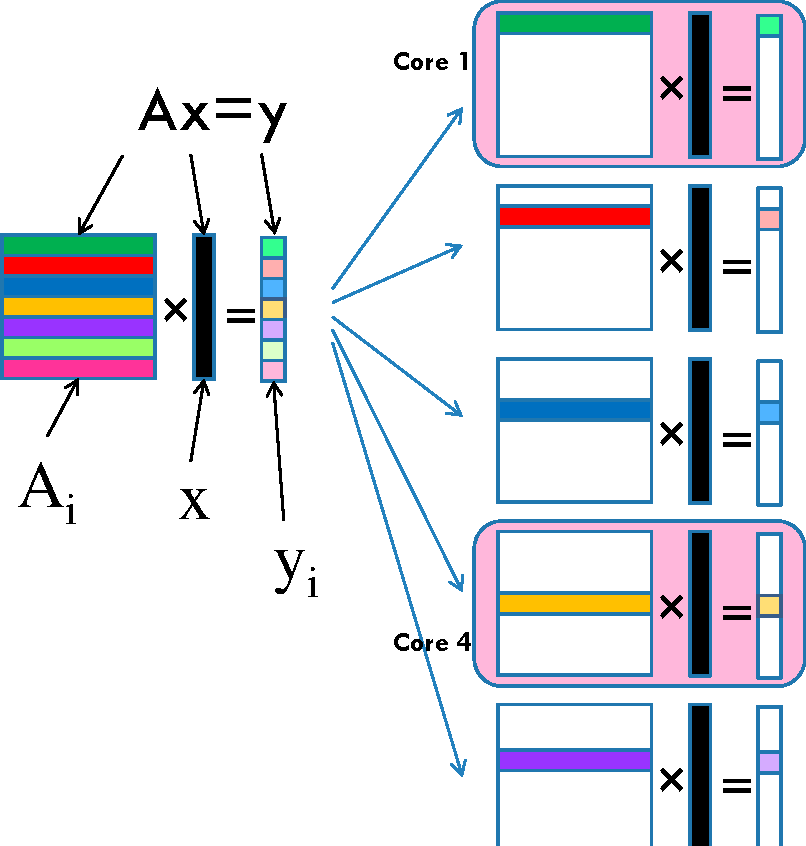
\includegraphics[width=.7\textwidth]{img/mvm-1.pdf}
    \caption{Example of MVM algorithm.}
\end{figure}

\newpage

\noindent
The performance of the MVM algorithm is as follows:
\begin{itemize}
    \item The \textbf{time to solve} a problem of size $n^{2}$ is equal to the big $O$ of the squared size of the problem as input divided by the number of processors available:
    \begin{equation*}
        T_{p}\left(n^{2}\right) = O\left(\dfrac{n^{2}}{p}\right)
    \end{equation*}
    
    \item The \textbf{cost} is equal to the number of processors and the time it takes to solve the problem. So it is quite trivial:
    \begin{equation*}
        C = O\left(\cancel{P} \cdot \dfrac{n^{2}}{\cancel{p}}\right) = O\left(n^{2}\right)
    \end{equation*}

    \item The \textbf{work} is equal to the cost, and the \textbf{linear power} $P$ is equal to the ratio of work and time to solve the problem on $p$ processors:
    \begin{equation*}
        W = C \hspace{2em} \dfrac{W}{T_{p}} = P
    \end{equation*}

    \item The \textbf{perfect efficiency} is equal to:
    \begin{equation*}
        E_{p} = \dfrac{T_{1}}{pT_{p}} = \dfrac{n^{2}}{p\frac{n^{2}}{p}} = 1
    \end{equation*}
\end{itemize}

    %%%%%%%%%%%%%%%%%%%%%%%%%%
    % Bibliography and index %
    %%%%%%%%%%%%%%%%%%%%%%%%%%
    \pagestyle{fancy}
\fancyhead{} % clear all header fields
\fancyhead[R]{\nouppercase{\leftmark}}

\bibliography{bibtex}{}
\bibliographystyle{plain}

\newpage

\printindex
\end{document}